\documentclass{beamer}

\usepackage[utf8]{inputenc}
\usepackage[T1]{fontenc}
\usepackage{adjustbox}
\usepackage{booktabs}
\usepackage{graphicx}
\usepackage{listings}
\usepackage{lstlinebgrd}
\usepackage{multirow}
\usepackage{subcaption}
\usepackage{tikz}
\usepackage{ulem}

\fontseries{bx}
\selectfont

\setlength{\tabcolsep}{18pt}

\graphicspath{{./gfx/}}

\usetikzlibrary{fit}

\usetheme{Madrid}

\title[Cloud MCS]{Improving Cloud Simulation Using the Monte-Carlo Method}
\author[Luke Bertot]{\underline{Luke Bertot} \and Stéphane Genaud \and Julien Gossa\\}
\institute[ICPS]{%
	\{lbertot,genaud,gossa\}@unistra.fr\\
	\medskip{}
	ICPS -- Scientific and Parallel Computing research group\\ 
	at ICube, University of Strasbourg CNRS}

\date[Euro-Par 2018]{Euro-Par, August 2018}

\titlegraphic{\raisebox{-0.5\height}{
\includegraphics[width=1.5cm]{/icube-png.png}}\hspace*{1cm}~\raisebox{-0.5\height}{
\includegraphics[width=2cm]{uds.png}}\hspace*{1cm}~\raisebox{-0.5\height}{
\includegraphics[width=1.5cm]{Logo_CNRS.png}}}

\setbeamertemplate{navigation symbols}{}%remove navigation symbols

\newcommand\blfootnote[1]{%
  \begingroup
  \renewcommand\thefootnote{}\footnote{#1}%
  \addtocounter{footnote}{-1}%
  \endgroup
}


\AtBeginSection[]{%
	\begin{frame}
		\begin{beamercolorbox}[sep=8pt,center,shadow=true,rounded=true]{title}
			\usebeamerfont{title}\insertsectionhead\par
		\end{beamercolorbox}
	 \end{frame}
}

\begin{document}

\begin{frame}
\maketitle{}
\end{frame}

\begin{frame}
	\frametitle{Outline}
	\tableofcontents
\end{frame}

\section{Cloud Brokering}

\begin{frame}
	\frametitle{Scientific Workloads}
	\resizebox{\textwidth}{!}{\usetikzlibrary{fit,arrows}
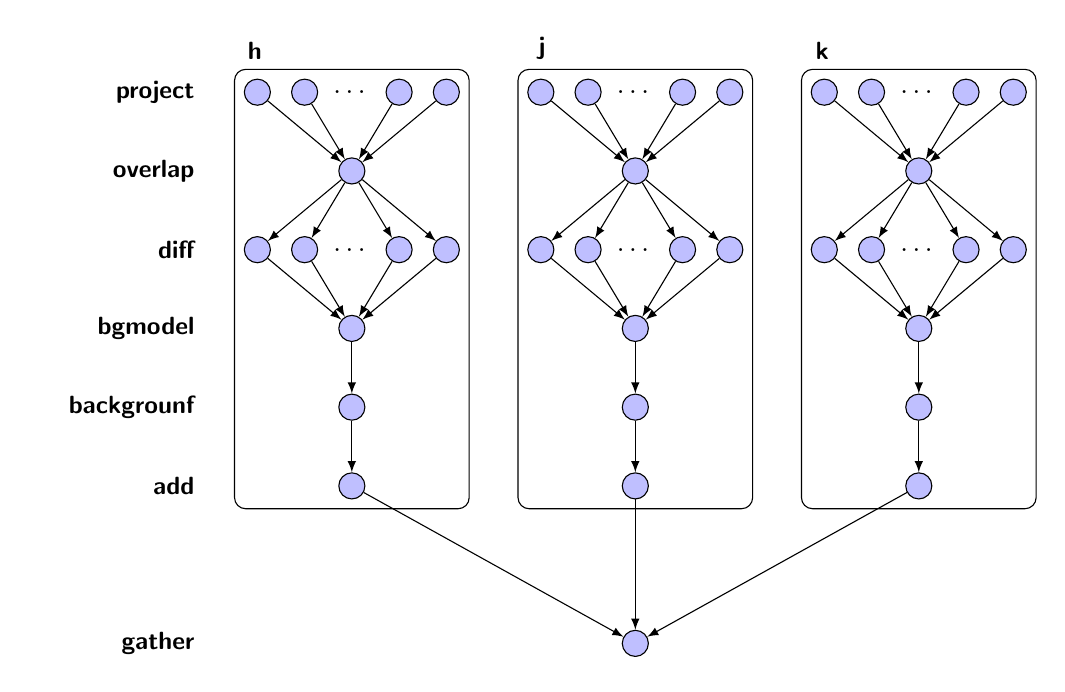
\begin{tikzpicture}[x=6mm,y=-10mm,
task/.style={%
 fill=blue!25,
draw,circle
},
level/.style={%
  font={\sffamily\bfseries\color{black} \fontsize{9pt}{12}\selectfont},
  align=right,
  text width=20mm
},
dot/.style={%
circle
}
]
%levels
\node[level] at (0,0)(Lproj){project};
\node[level] at (0,1)(Loverlap){overlap};
\node[level] at (0,2)(Ldiff){diff};
\node[level] at (0,3)(Lbgm){bgmodel};
\node[level] at (0,4)(Lbg){backgrounf};
\node[level] at (0,5)(Ladd){add};
\node[level] at(0,7)(Lgather){gather};
%%Gather node
\node[task,shift={(9,0)}]at(2,7)(gather){};
%%Loop HJK
\foreach \n [count=\i from 0] in {h,j,k}
{%
\begin{scope}[shift={(3+6*\i,0)}]
% 1 node per group
\node[task]at(2,1)(\i_overlap){};
\node[task]at(2,3)(\i_bgm){};
\node[task]at(2,4)(\i_bg){};
\node[task]at(2,5)(\i_add){};
%% 4 node per group
\foreach \y in {0,1,3,4}
{%
\node[task]at(\y,0)(\i_p_\y){};
\node[task]at(\y,2)(\i_d_\y){};
\draw[-{latex}](\i_p_\y)--(\i_overlap);
\draw[-{latex}](\i_overlap)--(\i_d_\y);
\draw[-{latex}](\i_d_\y)--(\i_bgm);
}
%%4 groups elipsis
\foreach \y in {0,2}
{%
\node[dot]at(2,\y){\ldots};
}
%%single deps
\draw[-{latex}](\i_bgm)--(\i_bg);
\draw[-{latex}](\i_bg)--(\i_add);
%%HJK boxes
\node[rounded corners,draw,fit=(\i_add)(\i_p_0)(\i_p_4),label={[font={\sffamily\bfseries\color{black}\fontsize{9pt}{12}\selectfont}]110:\n}]{};
\end{scope}
%% Gather deps
\draw[-{latex}](\i_add)--(gather);
}
\end{tikzpicture}}
%	preesent workflows we are working with.
\end{frame}

\begin{frame}
	\frametitle{Cloud Scheduling}
	\resizebox{\textwidth}{!}{\usetikzlibrary{fit}
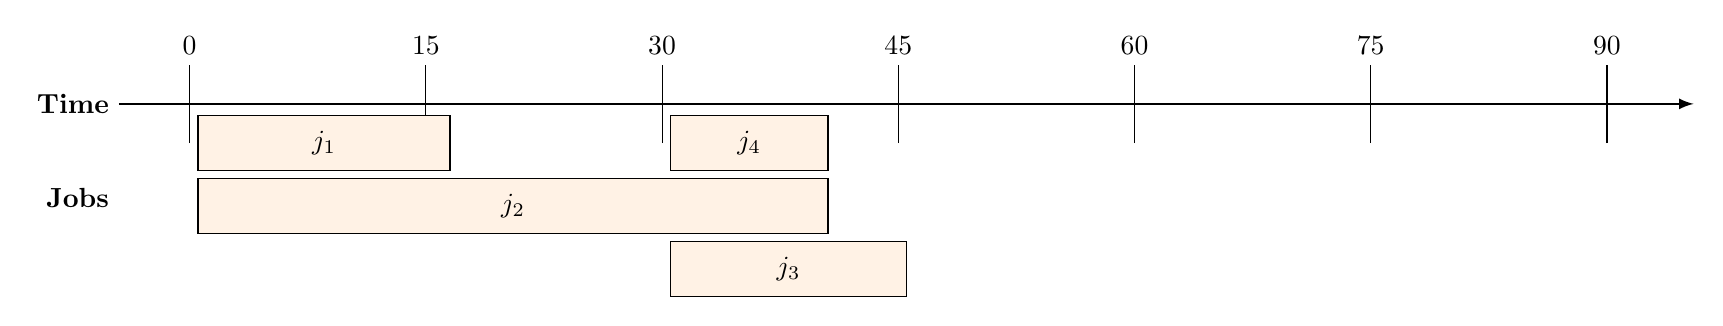
\begin{tikzpicture}[x=2mm,
job/.style={%
anchor=west,
fill=orange!10,
minimum height=7mm,
draw
},
btu/.style={%
anchor=west,
draw,
minimum height=9mm,
minimum width=120mm,
},
strat/.style={%
font=\bfseries,
anchor=east,
align=right,
},
]
%% Timeline
\node[strat]at(-5,0){Time};
\node[strat]at(-5,-1.2){Jobs};
\draw[-{latex},thick] (-5,0)--(95,0);
\foreach \x in {0,15,...,90}{%
\draw (\x-0.5,-0.5)--(\x-0.5,0.5) node[anchor=south]{\x};
}
%% Jobs
\node[job,minimum width=32mm]at(0,-0.5){$j_1$};
\node[job,minimum width=80mm]at(0,-1.3){$j_2$};
\node[job,minimum width=30mm]at(30,-2.1){$j_3$};
\node[job,minimum width=20mm]at(30,-0.5){$j_4$};
%\begin{scope}[shift={(0,2)}]
%% 1vm4all
%\node[strat]at(-5,0){1 VM for all};
%\node[job,minimum width=20mm]at(0,0){$j_1$};
%\node[job,minimum width=80mm]at(10,0){$j_2$};
%\node[job,minimum width=30mm]at(50,0){$j_3$};
%\node[job,minimum width=24mm]at(65,0){$j_4$};
%\node[btu,label={north:BTU 1}]at(-0.5,0){};
%\node[btu,label={north:BTU 2}]at(59.5,0){};
%\end{scope}
%\begin{scope}[shift={(0,4)}]
%% 1VM/job
%\node[strat]at(-5,1.5){1 VM per Job};
%\node[job,minimum width=20mm]at(0,3){$j_1$};
%\node[job,minimum width=80mm]at(0,2){$j_2$};
%\node[job,minimum width=30mm]at(30,1){$j_3$};
%\node[job,minimum width=24mm]at(30,0){$j_4$};
%\node[btu,label={east:BTU 1}]at(-0.5,3){};
%\node[btu,label={east:BTU 2}]at(-0.5,2){};
%\node[btu,label={west:BTU 3}]at(29.5,1){};
%\node[btu,label={west:BTU 4}]at(29.5,0){};
%\end{scope}
\end{tikzpicture}
} \\[1cm]
	\begin{overlayarea}{\textwidth}{.5\textheight}
		\only<2>{
			  \begin{itemize}
				\item bla blah 1
				\item bla blah 2
				\item bla blah 3
			  \end{itemize}
		}
		\only<3>{
		%\resizebox{!}{.5\textheight}{\input{img/gossiping.pdftex_t}}
		\resizebox{\textwidth}{!}{\usetikzlibrary{fit}
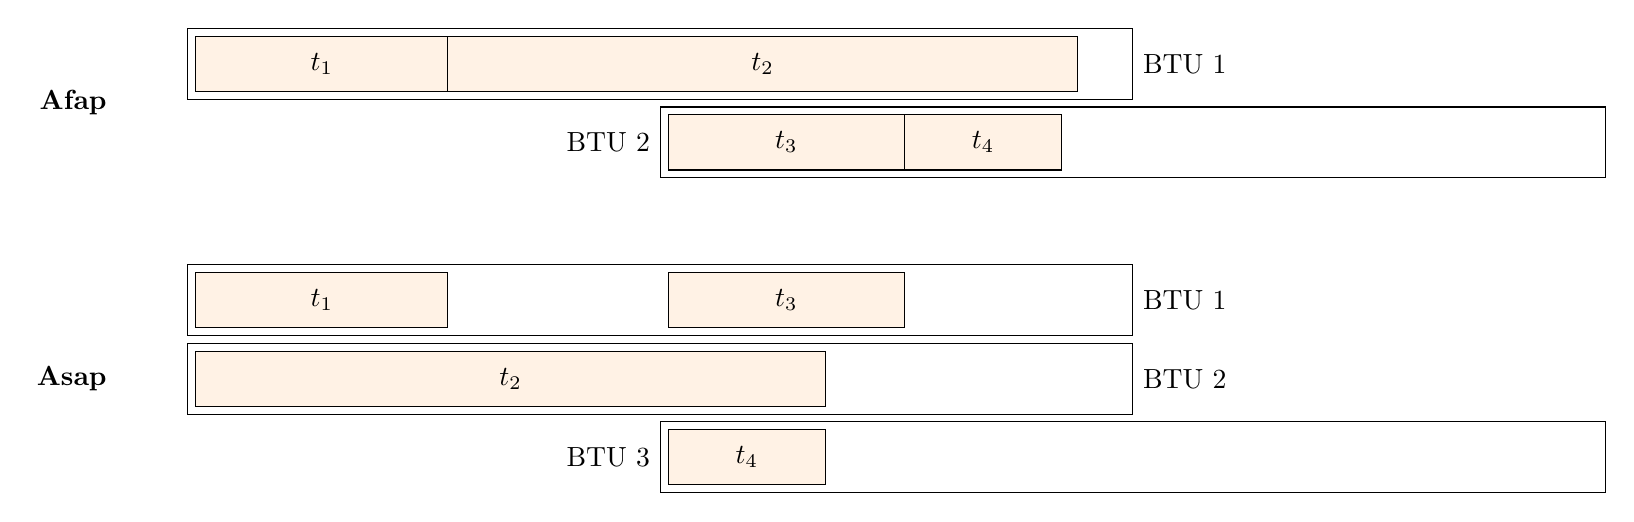
\begin{tikzpicture}[x=2mm,
job/.style={%
anchor=west,
fill=orange!10,
minimum height=7mm,
draw
},
btu/.style={%
anchor=west,
draw,
minimum height=9mm,
minimum width=120mm,
},
strat/.style={%
font=\bfseries,
anchor=east,
align=right,
},
]
%\begin{scope}[shift={(0,2)}]
%% 1vm4all
%\node[strat]at(-5,0){1 VM for all};
%\node[job,minimum width=20mm]at(0,0){$j_1$};
%\node[job,minimum width=80mm]at(10,0){$j_2$};
%\node[job,minimum width=30mm]at(50,0){$j_3$};
%\node[job,minimum width=24mm]at(65,0){$j_4$};
%\node[btu,label={north:BTU 1}]at(-0.5,0){};
%\node[btu,label={north:BTU 2}]at(59.5,0){};
%\end{scope}
%\begin{scope}[shift={(0,4)}]
%% 1VM/job
%\node[strat]at(-5,1.5){1 VM per Job};
%\node[job,minimum width=20mm]at(0,3){$j_1$};
%\node[job,minimum width=80mm]at(0,2){$j_2$};
%\node[job,minimum width=30mm]at(30,1){$j_3$};
%\node[job,minimum width=24mm]at(30,0){$j_4$};
%\node[btu,label={east:BTU 1}]at(-0.5,3){};
%\node[btu,label={east:BTU 2}]at(-0.5,2){};
%\node[btu,label={west:BTU 3}]at(29.5,1){};
%\node[btu,label={west:BTU 4}]at(29.5,0){};
%\end{scope}
\begin{scope}[shift={(0,-4)}]
%% Afap
\node[strat]at(-5,-.5)(f1){Afap};
\node[job,minimum width=32mm]at(0,0){$t_1$};
\node[job,minimum width=80mm]at(16,0){$t_2$};
\node[job,minimum width=30mm]at(30,-1){$t_3$};
\node[job,minimum width=20mm]at(45,-1){$t_4$};
\node[btu,label={east:BTU 1}]at(-0.5,-0)(f2){};
\node[btu,label={west:BTU 2}]at(29.5,-1)(f3){};
\end{scope}
\begin{scope}[shift={(0,-7)}]
%% Asap
\node[strat]at(-5,-1){Asap};
\node[job,minimum width=32mm]at(0,0){$t_1$};
\node[job,minimum width=80mm]at(0,-1){$t_2$};
\node[job,minimum width=30mm]at(30,0){$t_3$};
\node[job,minimum width=20mm]at(30,-2){$t_4$};
\node[btu,label={east:BTU 1}]at(-0.5,0){};
\node[btu,label={west:BTU 3}]at(29.5,-2){};
\node[btu,label={east:BTU 2}]at(-0.5,-1){};
\end{scope}
\end{tikzpicture}
}
		}
		\only<4>{
		%\resizebox{!}{.5\textheight}{\input{img/gossiping.pdftex_t}}
		\resizebox{\textwidth}{!}{\usetikzlibrary{fit}
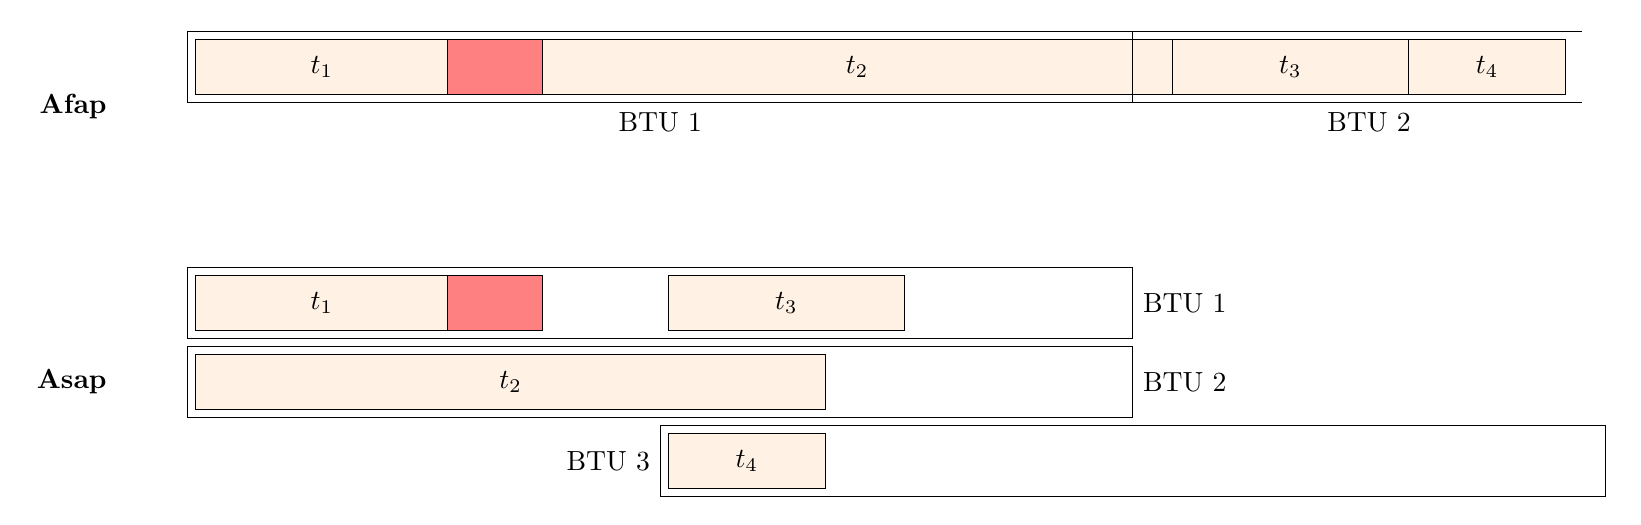
\begin{tikzpicture}[x=2mm,
job/.style={%
anchor=west,
fill=orange!10,
minimum height=7mm,
draw
},
over/.style={%
anchor=west,
fill=red!50,
minimum height=7mm,
draw
},
btu/.style={%
anchor=west,
draw,
minimum height=9mm,
minimum width=120mm,
},
strat/.style={%
font=\bfseries,
anchor=east,
align=right,
},
]
%\begin{scope}[shift={(0,2)}]
%% 1vm4all
%\node[strat]at(-5,0){1 VM for all};
%\node[job,minimum width=20mm]at(0,0){$j_1$};
%\node[job,minimum width=80mm]at(10,0){$j_2$};
%\node[job,minimum width=30mm]at(50,0){$j_3$};
%\node[job,minimum width=24mm]at(65,0){$j_4$};
%\node[btu,label={north:BTU 1}]at(-0.5,0){};
%\node[btu,label={north:BTU 2}]at(59.5,0){};
%\end{scope}
%\begin{scope}[shift={(0,4)}]
%% 1VM/job
%\node[strat]at(-5,1.5){1 VM per Job};
%\node[job,minimum width=20mm]at(0,3){$j_1$};
%\node[job,minimum width=80mm]at(0,2){$j_2$};
%\node[job,minimum width=30mm]at(30,1){$j_3$};
%\node[job,minimum width=24mm]at(30,0){$j_4$};
%\node[btu,label={east:BTU 1}]at(-0.5,3){};
%\node[btu,label={east:BTU 2}]at(-0.5,2){};
%\node[btu,label={west:BTU 3}]at(29.5,1){};
%\node[btu,label={west:BTU 4}]at(29.5,0){};
%\end{scope}
\begin{scope}[shift={(0,-4)}]
%% Afap
\node[strat]at(-5,-.5)(f1){Afap};
\node[job,minimum width=32mm]at(0,0){$t_1$};
\node[over,minimum width=12mm]at(16,0){};
\node[job,minimum width=80mm]at(22,0){$t_2$};
\node[job,minimum width=30mm]at(62,0){$t_3$};
\node[job,minimum width=20mm]at(77,0){$t_4$};
\node[btu,label={south:BTU 1}]at(-0.5,0)(f2){};
\node[btu,minimum width=60mm,label={south:BTU 2}]at(59.5,0)(f3){};
\node[anchor=west,minimum height=10mm,minimum width=4mm,fill=white]at(88,0){};
\end{scope}
\begin{scope}[shift={(0,-7)}]
%% Asap
\node[strat]at(-5,-1){Asap};
\node[job,minimum width=32mm]at(0,0){$t_1$};
\node[over,minimum width=12mm]at(16,0){};
\node[job,minimum width=80mm]at(0,-1){$t_2$};
\node[job,minimum width=30mm]at(30,0){$t_3$};
\node[job,minimum width=20mm]at(30,-2){$t_4$};
\node[btu,label={east:BTU 1}]at(-0.5,0){};
\node[btu,label={west:BTU 3}]at(29.5,-2){};
\node[btu,label={east:BTU 2}]at(-0.5,-1){};
\end{scope}
\end{tikzpicture}
}
		}
	\end{overlayarea}
\end{frame}

%\begin{frame}
%	\frametitle{Variability in Cloud environments}
%	\resizebox{\textwidth}{!}{\usetikzlibrary{fit}
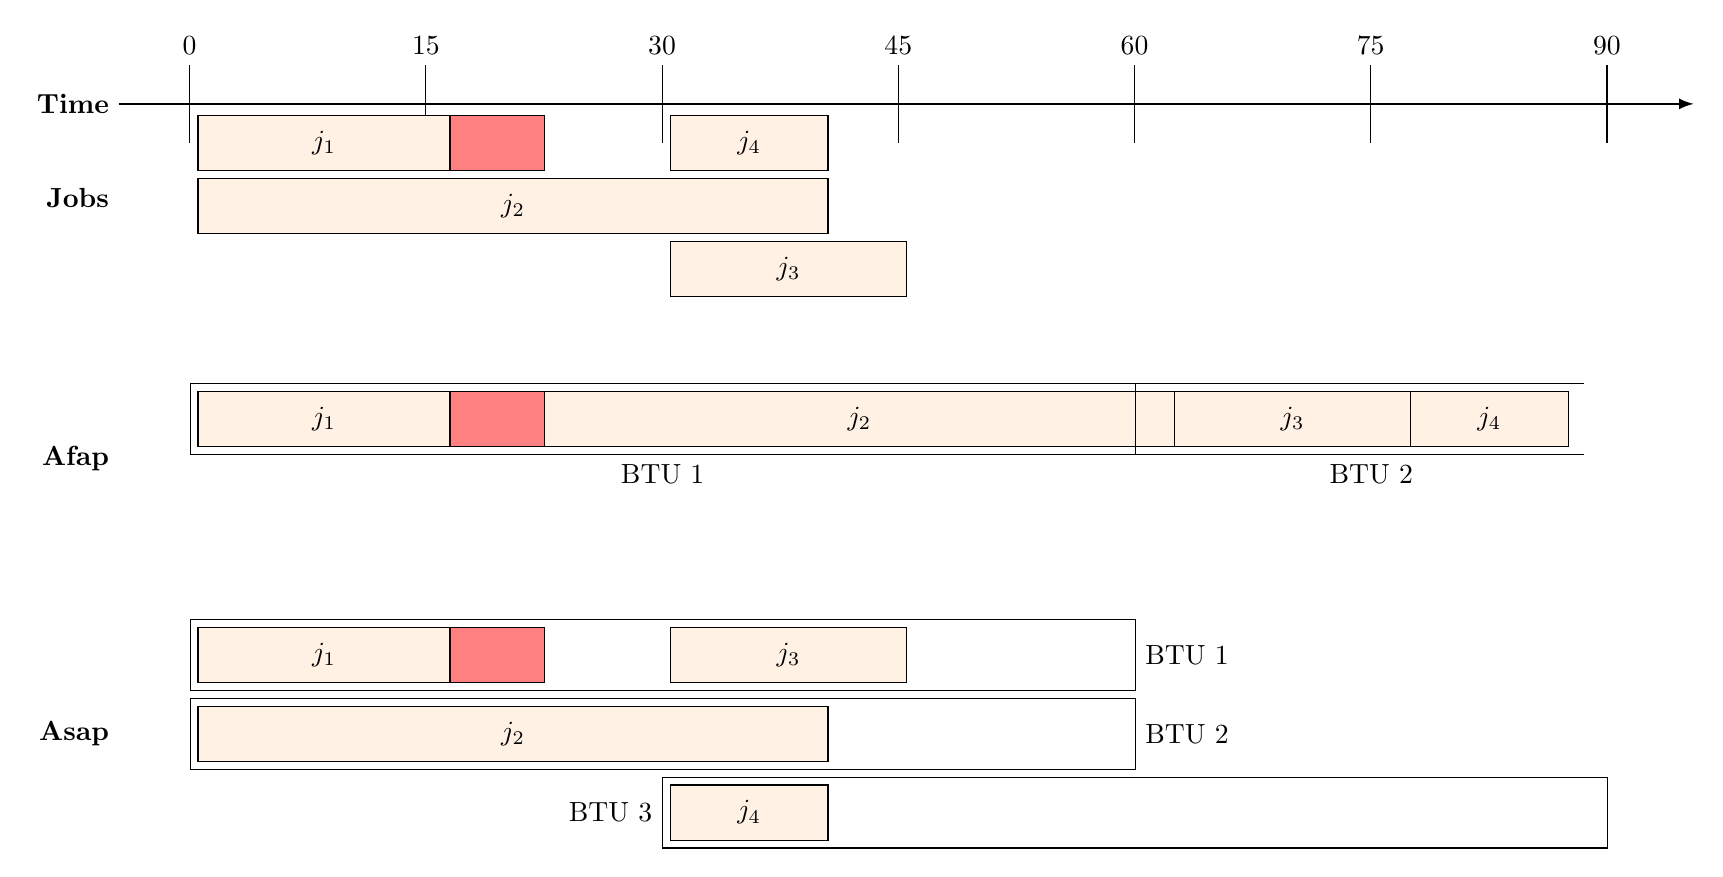
\begin{tikzpicture}[x=2mm,
job/.style={%
anchor=west,
fill=orange!10,
minimum height=7mm,
draw
},
over/.style={%
anchor=west,
fill=red!50,
minimum height=7mm,
draw
},
btu/.style={%
anchor=west,
draw,
minimum height=9mm,
minimum width=120mm,
},
strat/.style={%
font=\bfseries,
anchor=east,
align=right,
},
]
%% Timeline
\node[strat]at(-5,0){Time};
\node[strat]at(-5,-1.2){Jobs};
\draw[-{latex},thick] (-5,0)--(95,0);
\foreach \x in {0,15,...,90}{%
\draw (\x-0.5,-0.5)--(\x-0.5,0.5) node[anchor=south]{\x};
}
%% Jobs
\node[job,minimum width=32mm]at(0,-0.5){$j_1$};
\node[over,minimum width=12mm]at(16,-0.5){};
\node[job,minimum width=80mm]at(0,-1.3){$j_2$};
\node[job,minimum width=30mm]at(30,-2.1){$j_3$};
\node[job,minimum width=20mm]at(30,-0.5){$j_4$};
%\begin{scope}[shift={(0,2)}]
%% 1vm4all
%\node[strat]at(-5,0){1 VM for all};
%\node[job,minimum width=20mm]at(0,0){$j_1$};
%\node[job,minimum width=80mm]at(10,0){$j_2$};
%\node[job,minimum width=30mm]at(50,0){$j_3$};
%\node[job,minimum width=24mm]at(65,0){$j_4$};
%\node[btu,label={north:BTU 1}]at(-0.5,0){};
%\node[btu,label={north:BTU 2}]at(59.5,0){};
%\end{scope}
%\begin{scope}[shift={(0,4)}]
%% 1VM/job
%\node[strat]at(-5,1.5){1 VM per Job};
%\node[job,minimum width=20mm]at(0,3){$j_1$};
%\node[job,minimum width=80mm]at(0,2){$j_2$};
%\node[job,minimum width=30mm]at(30,1){$j_3$};
%\node[job,minimum width=24mm]at(30,0){$j_4$};
%\node[btu,label={east:BTU 1}]at(-0.5,3){};
%\node[btu,label={east:BTU 2}]at(-0.5,2){};
%\node[btu,label={west:BTU 3}]at(29.5,1){};
%\node[btu,label={west:BTU 4}]at(29.5,0){};
%\end{scope}
\begin{scope}[shift={(0,-4)}]
%% Afap
\node[strat]at(-5,-.5)(f1){Afap};
\node[job,minimum width=32mm]at(0,0){$j_1$};
\node[over,minimum width=12mm]at(16,0){};
\node[job,minimum width=80mm]at(22,0){$j_2$};
\node[job,minimum width=30mm]at(62,0){$j_3$};
\node[job,minimum width=20mm]at(77,0){$j_4$};
\node[btu,label={south:BTU 1}]at(-0.5,0)(f2){};
\node[btu,minimum width=60mm,label={south:BTU 2}]at(59.5,0)(f3){};
\node[anchor=west,minimum height=10mm,minimum width=4mm,fill=white]at(88,0){};
\end{scope}
\begin{scope}[shift={(0,-7)}]
%% Asap
\node[strat]at(-5,-1){Asap};
\node[job,minimum width=32mm]at(0,0){$j_1$};
\node[over,minimum width=12mm]at(16,0){};
\node[job,minimum width=80mm]at(0,-1){$j_2$};
\node[job,minimum width=30mm]at(30,0){$j_3$};
\node[job,minimum width=20mm]at(30,-2){$j_4$};
\node[btu,label={east:BTU 1}]at(-0.5,0){};
\node[btu,label={west:BTU 3}]at(29.5,-2){};
\node[btu,label={east:BTU 2}]at(-0.5,-1){};
\end{scope}
\end{tikzpicture}
}
%\end{frame}

\begin{frame}
	\frametitle{The Schlouder cloud broker}
	\resizebox{\textwidth}{!}{\usetikzlibrary{fit,arrows}
\begin{tikzpicture}[node distance=5pt,x=25mm+5pt,y=15mm+5pt,
every node/.style={anchor=center,
line width=1pt,
minimum width = 25mm,
minimum height =15mm,
rounded corners,
label distance=-5mm,
draw 
},
high/.style={%
minimum height =45mm+10pt,
},
large/.style={%
minimum width=50mm+5pt
}]
\node[high]at(0,0)(app){Schlouder};
\node[]at(1,-1)(ck){CloudKit};
\node[]at(1,0)(strat){Strategy};
\node[]at(1,1)(slm){Slurm};
\node[align=center]at(3,-1)(cc){Openstack\\frontend};
\node[]at(3,0)(vm1){VM};
\node[]at(3,1)(vm2){VM};
\node[draw,fit=(app)(ck)(slm),label={below:Cloud Broker}]{};
\node[draw,fit=(vm2)(cc)(vm1),label={below:Cloud}]{};
\draw [{triangle 45}-{triangle 45},line width=2pt] (ck)--(cc);
\draw [{triangle 45}-{triangle 45},line width=2pt] (vm2)--(slm);
\draw [{triangle 45}-{triangle 45},line width=2pt] (vm1)--(slm);
%\draw [{triangle 45}-{triangle 45},shorten <=10pt,shorten >=10pt] (1,0)--(1,1);
%\draw [{triangle 45}-{triangle 45},shorten <=10pt,shorten >=10pt] (1,0)--(1,-1);
\end{tikzpicture}
}
	%( present schlouder ) 
\end{frame}


%\section{Cloud Simulations}

\begin{frame}
	\frametitle{SimSchlouder}
	\resizebox{\textwidth}{!}{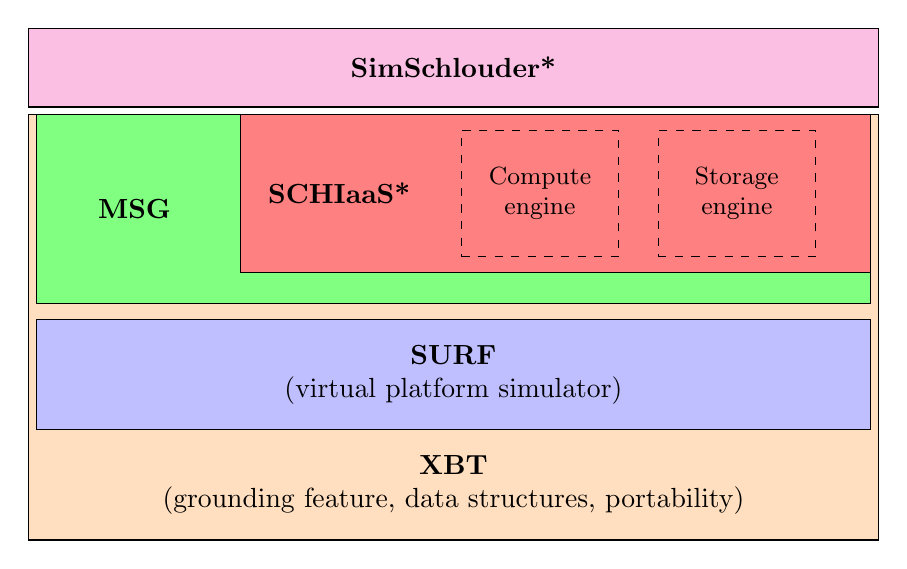
\begin{tikzpicture}[x=1cm,y=1cm,
every node/.style={
rectangle,
align = center,
anchor=south west,
outer sep=1mm,
},
box/.style={
draw,
}]

%Simgrid box
\node[box,minimum height=5.4cm,minimum width=10.8cm,fill=orange!25,
%label={south:\small{}\textsf{\textbf{SimGrid}}}
]at(0,0){};
%\node[box,minimum height=5.8cm,minimum width=1.4cm,fill=cyan!50]at(11,0){\rotatebox{270}{\textbf{Tracing}}};
\node[minimum height=1.4cm,minimum width=10.6cm]at(0.1,0){\textbf{XBT}\\(grounding feature, data structures, portability)};
\node[box,minimum height=1.4cm,minimum width=10.6cm,fill=blue!25]at(0.1,1.4){\textbf{SURF}\\(virtual platform simulator)};
\node[box,minimum height=2.4cm,minimum width=10.6cm,fill=green!50]at(0.1,3){};
\node[minimum height=2.4cm,minimum width=2.5cm]at(0.1,3){\textbf{MSG}};
\node[box,fill=red!50,minimum height=2cm,minimum width=8cm]at(2.7,3.4){};
\node[minimum height=2cm,minimum width=2.5cm]at(2.7,3.4){\textbf{SCHIaaS*}};
\node[box,dashed,minimum height=1.6cm,minimum width=2cm]at(5.5,3.6){};
\node[anchor=center,font=\small]at(6.6,4.5){Compute\\engine};
\node[box,dashed,minimum height=1.6cm,minimum width=2cm]at(8,3.6){};
\node[anchor=center,font=\small]at(9.1,4.5){Storage\\engine};
\node[box,fill=magenta!25,minimum width=10.8cm,minimum height=1cm]at(0,5.5){\textbf{SimSchlouder*}};
\end{tikzpicture}}
	%present simschlouder limits to that approach
\end{frame}

\begin{frame}
	\frametitle{Stochastic Simulations}
	??? bulletpoints
\end{frame}

\section{Monte-Carlo Simulations}

\begin{frame}
	\frametitle{Monte Carlo Simulations}
	\resizebox{\textwidth}{!}{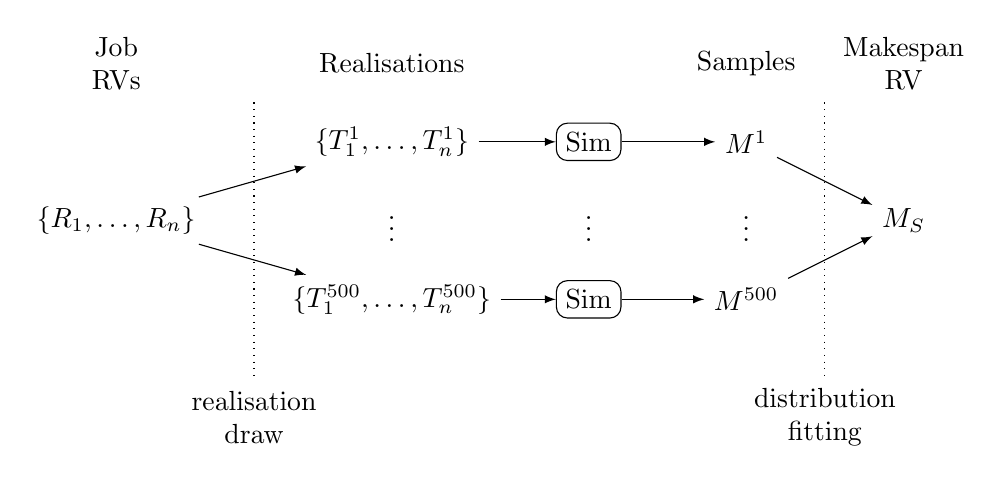
\begin{tikzpicture}[
sim/.style={%
draw, 
rounded corners
}
]
%% Origin node
\node[align=center]at(0,2){Job\\RVs};
\node at(0,0)(orig){$\{R_1,\ldots,R_n\}$};
%% Realisations
\node at(3.5,2){Realisations};
\node[]at(3.5,1)(pert1){$\{T_1^1,\ldots,T_n^1\}$};
\node at(3.5,0){\vdots};
\node at(3.5,-1)(pert5){$\{T_1^{500},\ldots,T_n^{500}\}$};
\draw[-{latex}](orig)--(pert1);
\draw[-{latex}](orig)--(pert5);
%%
\node[sim]at(6,1)(s1){Sim};
\node[sim]at(6,-1)(s5){Sim};
\node at(6,0){\vdots};
\draw[-{latex}](pert1)--(s1);
\draw[-{latex}](pert5)--(s5);
%% Makespans
\node at(8,2){Samples};
\node at(8,1)(M1){$M^1$};
\node at(8,-1)(M5){$M^{500}$};
\node at(8,-0){\vdots};
\draw[-{latex}](s1)--(M1);
\draw[-{latex}](s5)--(M5);
%% Consolidation
\node[align=center]at(10,2){Makespan\\RV};
\node at(10,0)(r){$M_S$};
\draw[-{latex}](M1)--(r);
\draw[-{latex}](M5)--(r);
%%phases
\node[align=center]at(1.75,-2.5)(df){realisation\\draw};
\draw[dotted](1.75,1.5)--(1.75,-2);
\node[align=center]at(9,-2.5)(df){distribution\\fitting};
\draw[dotted](9,1.5)--(9,-2);
\end{tikzpicture}
}
\end{frame}

\begin{frame}
	Experimental rational	(+modele simple)
\end{frame}

\begin{frame}
	our experimental setup (in vivo/in silico)
\end{frame}

\begin{frame}
	\frametitle{In-Vivo observations}
	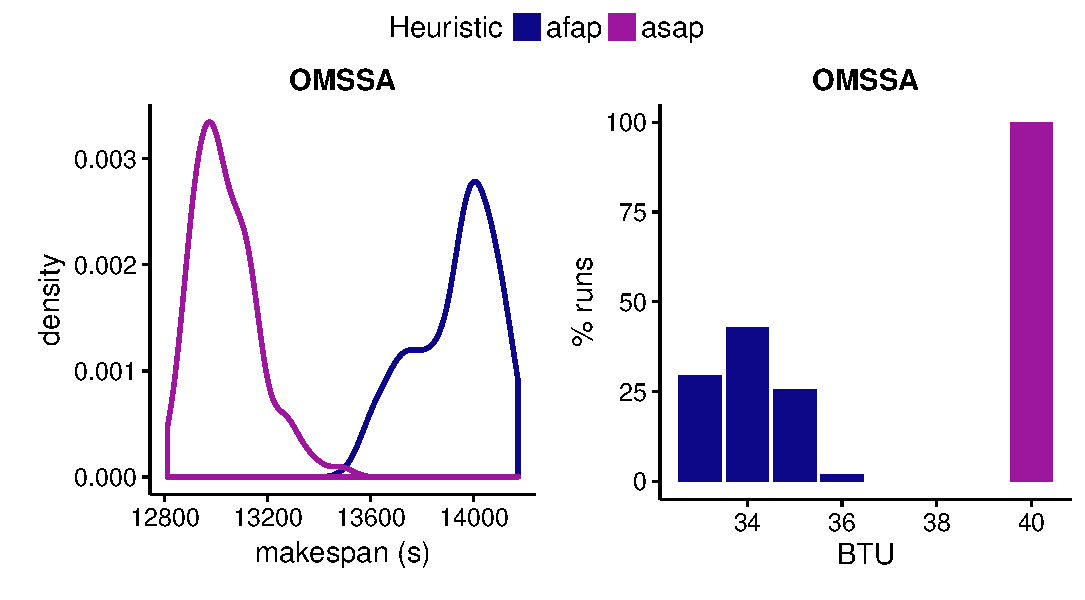
\includegraphics[width=\textwidth]{gfx/real.pdf}
\end{frame}

\begin{frame}
 	input model +(Leitner)
\end{frame}

\section{Results}

\begin{frame}
	\frametitle{Simulation Results}
	\begin{center}
	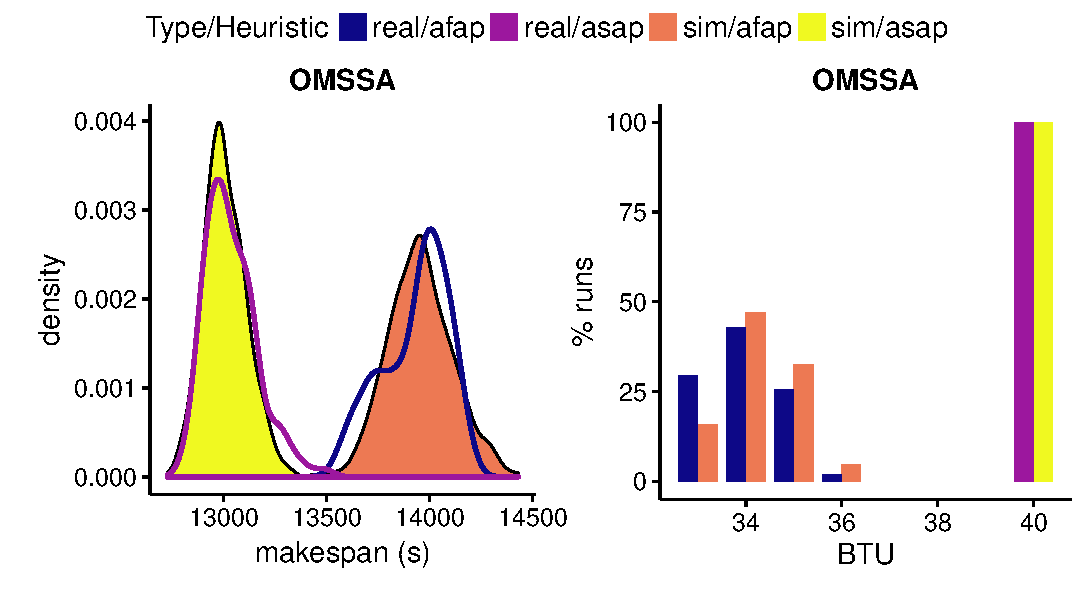
\includegraphics[height=0.6\textheight]{gfx/fit.pdf}\\
	{\small
	\begin{tabular}{lccc}
		\toprule
		Heuristic~&\multicolumn{2}{c}{~Makespan (Size of
		CI)~}&~BTU\\
		 & CI 95\% & CI 99\% &\\
		\midrule
		ASAP& 90\% (3\%)& 98\% (5\%)& 100\%\\
		AFAP& 92\% (4\%)& 100\% (6\%)& 100\%\\
		\bottomrule
	\end{tabular}
	}
	\end{center}
\end{frame}

\begin{frame}
	\frametitle{???}
	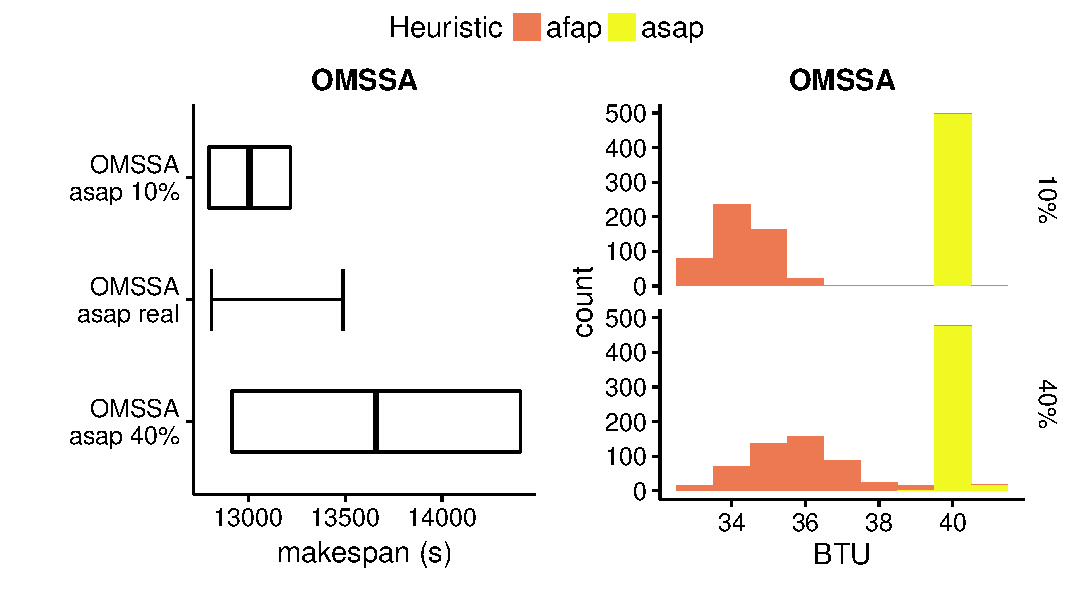
\includegraphics[width=\textwidth]{gfx/int.pdf}
\end{frame}

\begin{frame}
	number iter
\end{frame}
\section{conclusion}
\end{document}
% vim: spell spelllang=en
